\subsection{Network of Agents}\label{subsec:network}
Our network is made of agents eventually connected by weighted and
undirected edges. The network is composed by of a fixed number of
sources and users.\\
Users are tied with a attachment probability computed from the desired average
degree and inserted by external input. In this way we obtain a random
network of users, with exponential trend for the degree distribution in
the termodynamical limit. We can see intial degree distribution in linear scale 
(figure~\ref{fig:gauss}).
%
\begin{figure}[!h]
  \centering
  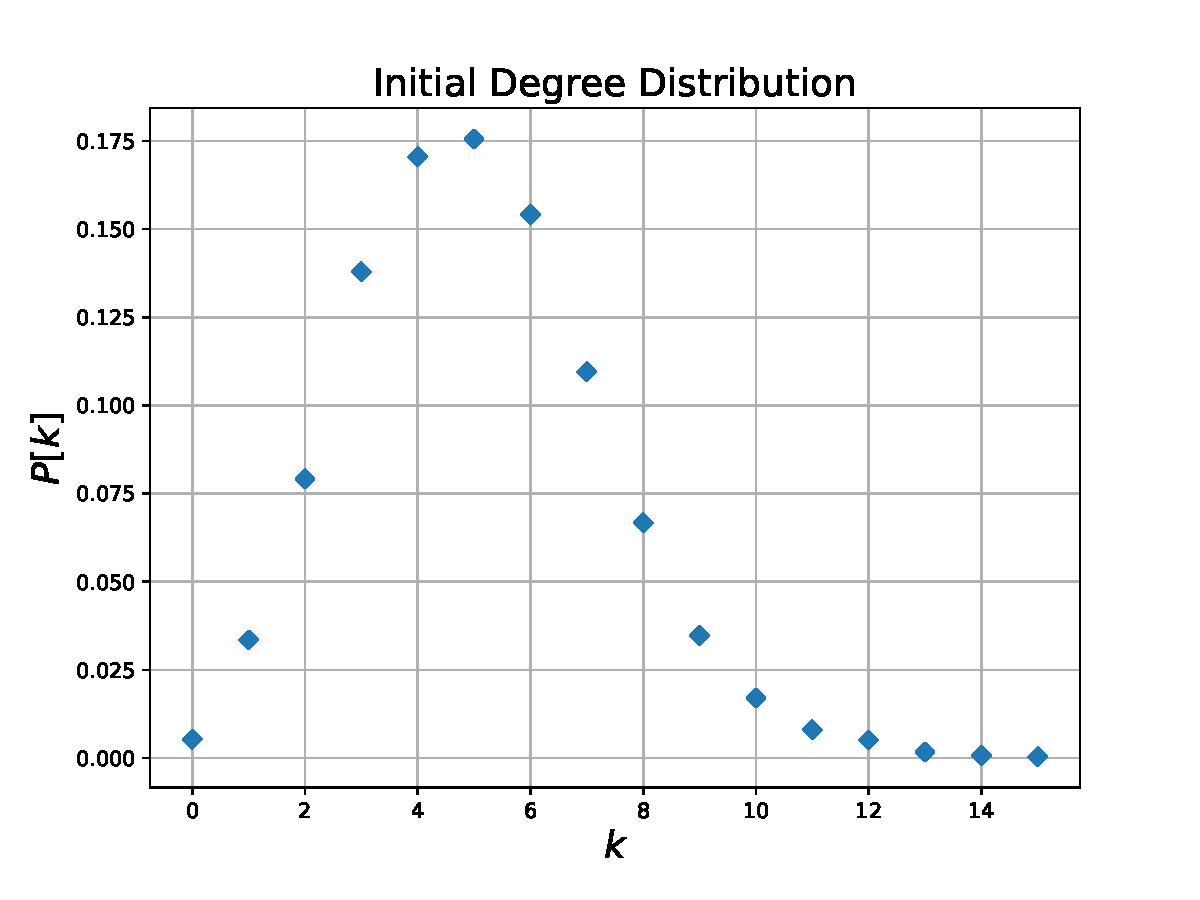
\includegraphics[width=.7\columnwidth]{img/pdf/gauss.pdf}
  \caption{Degree Distribution, seed 17, 3 sources, 10000 users, 5 initial average degree, 1 time step}
  \label{fig:gauss}
\end{figure}
%
\\
Links are the only possibility to establish a relation between the agents;
a random value of edge's weight represents a previous bias in
friendship.\footnote{This particular choice for our links underlines
  bilaterality and intensity of communication between agents. Taking
  as example an exchange of information between two people or between a
  person and a newspaper, weight represents feeling, previous chemistry;}
The result of such a mechanism of graph generation doesn't actually return
a real network, because social real networks possess the property of 
scale-free,\footnote{The scale-free property is mainly described by power
  law degree distribution, with a cut-off for high degrees (i.e. hubs). }
instead, in random graphs, the majority of node-degree is near the
average-degree.
Furthermore, in scale-free network, variance is very large and guarantees
the existence of hubs in the network.\cite{newman1963introduction}
Despite the abovementioned theory, we start with a random network hoping
to observe a natural evolution in this direction.

Sources are a news reservoir: users can pick one or more news from them
and eventually spread. Sources' degree is higher than users' one
because we assume that newspapers have more links than a common user. Sources
contain a fixed number of news and eventually create fresh news run-time.\\
Each single news contains a unique string which identifies it, a vector
of topics, the initial source's ID, creation date, its own relevance
(a sort of "impact factor").

Users inculde the "state of mind", a vector representing their own personality;
sources, like users, have a "personality" too (i.e. another vector)
which reflects news' content.
Users can remember a limited number of news, according to the affinity
between incoming news and their state of mind.
Furthermore, affinity also regulates diffusion among users.
State of mind is not fixed since is affected by news spreading;
edges' weights can be modified by users' state of mind.
Time is externally imposed and, according to it, users can be active
or inactive: they can interact with external world when active.
